\chapter{Related Work}
\section{GPU Application Characterization}
Since GPGPU computing exists, there are publications characterizing GPU application. This happens usually on
two levels. Either, the whole application, with all it's kernels and iterations is examined, or low-level 
features like branch divergence or cache misses are subject to the research.

Works like \cite{}, \cite{} or  \cite{} broadly analyse whole applications on a superficial level, without looking at the interactions of different elements inside the application. Metrics used are ...

Publication like \cite{} or \cite{} focus on the impact of architectural changes on applications. The paper \cite{} focusses on the impact of the dynamic parallelism on GPU workloads. 
However, to the best  knowledge of the author, there are no publication researching intra-application communication.
%\begin{itemize}
%	\item Usually see Application not as a set of different kernels and ignore kernel "interactions"...
%	\item ... or go down to instruction/warp 
%	\item ... or look at architectural impacts on applications
%	\item A Characterization and Analysis of PTX Kernels
%	Andrew Kerr, Gregory Diamos, and Sudhakar Yalamanchili: Broad overview on many applications. Simulated PTX execution, Memory Intesity, branch divergence etc.
%	\item Most other Papers analyse on similar levels, focussing on different Application or Architecture Aspects
%\end{itemize}
\section{GPU Code Instrumentation}
Instrumenting existing application with addition code for memory tracing is essential for this work.
A framework for code instrumentation is presented in "Lynx: A Dynamic Instrumentation System for Data-Parallel Applications on GPGPU Architectures" \cite{lynx} by ... . Lynx is a framework including a C-to-PTX JIT, that extends CUDA code on PTX instruction level and a runtime, displayed in \ref{lynx-rt}. The user writes instrumentation specification in a C-style language. The specification is translated to PTX and inserted into the original application.

The application can be instrumented on kernel, basic block and instruction level. An API offers access to CUDA constructs like Thread and CTA IDs, CTA barriers and instruction counts. To increase
efficiency, it is possible that only one thread in a warp performs the specified trace operation. It is possible to access shared and global memory space. The runtime fetches all generated data from the device after the application has finished.

There are two reasons, Lynx is not suitable for this project. First, while it is possible to instrument global memory operations, we found no way to access details about the instrumented instruction, like target address or type size. However, address information is crucial for this work. The second reason
is the runtime handling the data buffers. As the generated trace data can be very big, device memory would not suffice to hold all the data, and creating a dynamic producer-consumer buffer using Lynx seemed not feasible. 
\begin{figure}[t]
	\centering
	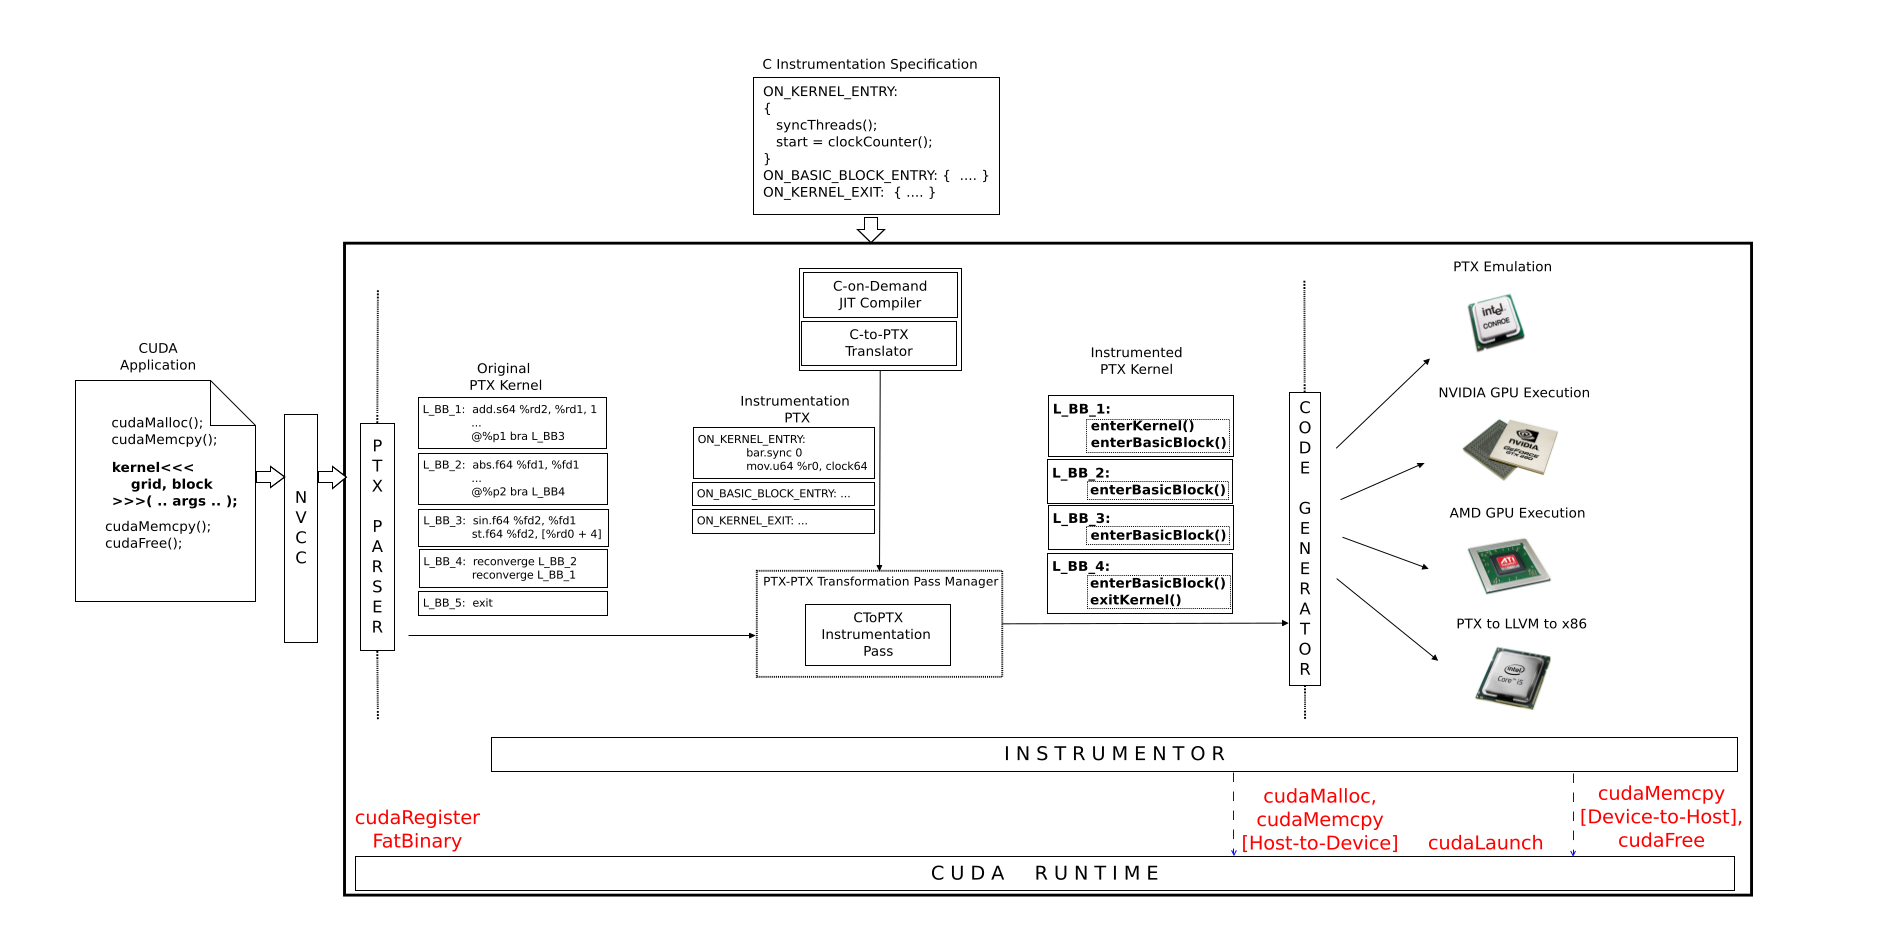
\includegraphics[trim={2.5cm 0 4cm 0},clip,width=\textwidth]{lynx-rt}
	\caption{Lynx framework with all components. The original application is instrumented on PTX level, with code generated by a C-to-PTX JIT from instrumentation specification. Generated data is moved and form the device by the runtime.}
	\label{lynx-rt}
\end{figure}
%\section{MPI Communication Traces}
%\begin{itemize}
%	\item Not the same because Message Passing != Shared Memory
%	\item Communication Patterns: Rolf Riesen: Paper on Communication Analysis and Patterns, not focussing on special Applications or Architectures. Provides useful metrics to discuss communication
%\end{itemize}